In diesem Kapitel beschreiben wir die geleistete Implementierungsarbeit im
Detail. Wir trennen die Änderungen dabei in bei FIFE und bei UH geleistete
Arbeit auf, wobei der Fokus auf UH liegt. 


\subsection{Kommandozeilen-Parameter (FIFE)}
Normalerweise sucht der FIFE-Editor Plugins nur in einem Unterordner relativ zu
seinem Ordner. Dort können Plugins aus UH naturgemäß nicht abgelegt werden. Wir
benötigen daher einen Kommandozeilen-Parameter {\tt --plugin-dir=PLUGIN\_DIR},
der es ermöglicht, manuell einen PATH zum Durchsuchen auf Plugins vorzugeben. 

Da der FIFE-Filbrowser kaum benutzbar ist, und um ein schnelles Laden von Karten
ohne viele Benutzerinteraktionen zu ermöglichen, implementierten wir im FIFE
Editor die Möglichkeit, Karten mittels Kommandozeilenargument zu laden. 



\subsection{Schaffung der Plugin-Infrastruktur (FIFE)}
Die Saver-Infrastruktur musste zunächst über das Anlegen mehrer C++
``Interfaces'' grundsätzlich in FIFE bereitgestellt werden. Erst dann standen
diese via SWIG (cf.
\cite{swig}) auch im Python-Teil von FIFE zur Verfügung. Damit konnte dann in
Python die Infrastruktur zum Registrieren von beliebigen MapSavers geschaffen
werden.

\subsection{Das Kartenformat}
\label{kartenformat}

%
% algorithm principle
%
\begin{figure}[htbp]
  \centering

    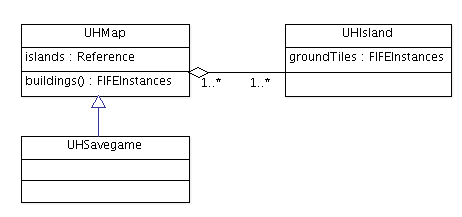
\includegraphics[width=0.7\textwidth]{gfx/klassendiagramm-UHSaveGame.png}

  \caption{UML Diagramm des Kartenformates von UH.}
  \label{figure:automaton-intersection}
\end{figure}

UHs Kartenformat in SQLite besteht grob aus den folgenden für den
Editor relevanten Elementen:
\begin{itemize}
  \item Allgemeinen Karteninformationen
  \item Die auf der Karte plazierten Objekte (wie Gebäude etc.)
  \item Verweise auf Island-Files. \\
  Ein Island-File ist eine SQLite-Datenbank,
  die die Informationen über die Bodenbeschaffenheit einer zusammengehörenden
  Inseln enthält:
  \begin{itemize}
    \item Allgemeine Islandinformationen
    \item Alle zu einem Island gehörenden Groundtiles
  \end{itemize}
\end{itemize}


\subsection{Plugin zum Laden von UH Objekten (UH)}
UH speichert alle dem Spiel zur Verfügung stehenden Objekte in mehreren Dateien
und Verzeichnissen:

\begin{description}
\item[content/objects] Dieser Ordner enthält mehrere Unterordner, die wiederum
YAML-Dateien\footnote{Ein Dateiformat, siehe \cite{yaml}} enthalten. Jede
dieser Dateien definiert ein Objekt und seine zugehörigen Eigenschaften.
\item[content/gfx] Dieser Ordner enthält die Grafiken, die zu den Objekten
gehören. Dabei sind die Grafiken für animierte Objekte auf mehrere Dateien
aufgeteilt, die in sogenannte ActionSets gruppiert werden.
\end{description}

UH bietet Klassen an, um diese Daten einzulesen.
Mithilfe dieser Klassen war es uns möglich, ein
Plugin für den FIFE Editor zu erstellen, das alle Gebäude und Bodentiles
laden und dem Editor zur Verfügung stellen kann.

Es war jedoch vonnöten, einige UH-Klassen vom Editor aus zu
modifizieren oder nachzuahmen, da die genutzten Klassen teilweise
globale Objekt erwarten, die das Spiel bereitstellt, die im Editor
jedoch nicht vorhanden sind.

Das Plugin besteht aus einer einzigen Klasse: \code{UHObjectLoader}. Diese
Klasse wird vom Editor geladen und anschließend wird ihre \code{enable()} Methode
aufgerufen. Diese lädt anschließend erst alle Groundtiles und dann alle Gebäude.
Sobald die Objekte der Engine bekannt sind, können diese mittels der vom Editor
bereitgestellten Werkzeuge auf Maps platziert werden.

\subsubsection{Groundtiles}
Um die Groundtiles zu laden wird die UH-Klasse \code{GroundTileLoader} benutzt,
die alle vorhandenen Groundtiles einliest und als Liste zurückgibt. Anschließend
wird für jedes der Tiles ein \code{Object} und ein \code{InstanceVisual} in der
Engine erstellt, sowie mehrere \code{Action}s und \code{ActionVisual}s, um Animationen darzustellen.
Alle diese Objekte benötigt die Engine, um die Tiles später im Editor korrekt
darstellen zu können.

\subsubsection{Gebäude}
Für die Gebäude müssen zunächst die XML-Deskriptoren ausgelesen werden, die
zusätzliche Informationen zu jedem Gebäude enthalten, wie z.B. dessen Größe.

Anschließend werden wiederum ein \code{Object}, \code{InstanceVisual} und
mehrere \code{Action}s und \code{ActionVisual}s erstellt, um das Gebäude in
der Engine zu registrieren.


\subsection{Plugin zum Laden von UH Karten (UH)}
\label{sec:registerMapLoader}
Um eine Map mit dem FIFE Editor öffnen zu können, muss zunächst die
Dateierweitung mit einem sogenannten \code{MapLoader} verknüpft werden.
Hierzu wird folgender Code
aufgerufen, der die Klasse \code{MapLoader} des \code{UHMapLoader} Plugins
als Loader für Dateien mit der Erweiterung \code{.sqlite} registriert:

\begin{lstlisting}
fife.extensions.loaders.addMapLoader('sqlite', UHMapLoader)
\end{lstlisting}

Sobald die daraufhin eine Map mit \code{.sqlite} Erweiterung im Editor geöffnet
wird, instantiiert dieser die \code{MapLoader} Klasse und ruft folgende Methode
auf:

\begin{lstlisting}
loadResource(self, path)
\end{lstlisting}

Daraufhin beginnt der \code{MapLoader} mit dem Einlesen der Map.

\subsubsection{Allgemeine Initialisierung}
Zunächst werden einige Map-unabhängige Initialisierung vorgenommen:
Der Loader erstellt eine \code{Map} in der Engine und darauf ein
\code{Grid}, auf dem später die einzelnen Tiles platziert werden.
Anschließend werden zwei \code{Layer} erstellt -- einer für Groundtiles
und einer für Gebäude. Dies ist notwendig, da die Engine pro Koordinate
und Layer nur ein Tile platzieren kann. D.h. wenn auf dem selben Layer
ein Gebäude über ein Groundtile platziert wird, so wird das Groundtile
überschrieben.
Abschließend wird noch eine \code{Camera} erstellt, die festlegt, aus
welcher Perspektive die Karte im Editor dargestellt wird.

\subsubsection{Inseln}
Als nächstes werden die Inseln der Map geladen. Hierzu wird zum ersten
Mal auf die SQLite Datenbank zugegriffen. Diese enthält eine Tabelle
namens \code{island}, die die Koordinaten jeder Insel enthalten, sowie
den Dateinamen der SQLite Datenbank, die die Inseldefinition enthält.

Für jede der ausgelesenen Inseln wird eine Subroutine aufgerufen, die
die Insel aus ihrer SQLite Datei ausliest. Hierbei werden aus der
\code{ground} Tabelle die Positionen und die Rotation der einzelnen
Groundtiles ausgelesen. Anschließend wird ein solches Groundtile
auf der \code{Map} in der Engine platziert.

Dies geschieht, indem eine \code{Instance} und ein \code{InstanceVisual}
erstellt werden. Die \code{Instance} speichert die Position des Tiles
auf der Map. Diese Position erhält man, wenn man die aus der Datenbank
gelesene Position des Tiles relativ zur Position der Insel verschiebt.

\subsubsection{Gebäude}
Um die Gebäude zu laden, wird aus der ursprünglichen Map-Datenbank
die Tabelle \code{building} ausgelesen. Diese enthält den Typ des Gebäudes,
sowie seine Position und Rotation.

Mit Hilfe dieser Informationen wird anschließend ein \code{Object}, eine
\code{Instance} und ein \code{InstanceVisual} erstellt. Abschließend
wird die \code{Instance} angewiesen, eine Animation auszuführen.

Beim Erstellen der Instance werden zum einen die Koordinaten des Gebäudes
gesetzt und zum andern das Gebäude rotiert. Dies ist ein aufwändiger
Prozess, da das Gebäude beim Rotieren wiederum verschoben wird.


\subsection{Plugin zum Speichern von UH Karten (UH)}
Um eine Map mit dem FIFE Editor öffnen zu können, muss
zunächst die Dateierweitung mit einem sogenannten \code{MapSaver} verknüpft
werden. Dieses Vorgehen ist analog zu Abschnitt~\ref{sec:registerMapLoader}. Die
dafür nötige Infrastruktur und wurde von uns wie in
Abschnitt~\ref{plugininfrastruktur} beschrieben in den FIFE-Editor
implementiert.

Registrieren des MapSavers

\begin{lstlisting}
fife.extensions.loaders.addMapLoader('sqlite', UHMapSaver)
\end{lstlisting}

Sobald die daraufhin eine Map mit \code{.sqlite} Erweiterung im Editor
gespeichert wird, instantiiert dieser die \code{UHMapLoader} Klasse und ruft
folgende Methode auf:

\begin{lstlisting}
saveResource(self, path)
\end{lstlisting}

Daraufhin beginnt der \code{UHMapSaver} mit dem Speichern der Map.

\subsubsection{Grundlegendes Speichern}
Grundsätzlich untergliedert sich das Speichern in die folgenden Schritte:
\begin{itemize}
  \item Speichern der Informationen des Ground-Layers
  \item Speichern der Informaitonen des Building-Layers
\end{itemize}

Die Layer-Schichten enthalten vor dem Speichern die Instanzen aller vom User
gesetzen Gebäude und Bodentiles.

Das Problem besteht nun darin, dass der Editor nicht die
Interna des UH Spielmodells kennen kann. Der Editor ``zeichnet'' einfach nur
Elemente wie Bodentiles und Gebäude auf die verschiedenen Layer-Schichten, das
Saver-Plugin muss diese in ein gültiges UH-Model umwandeln.

\subsubsection{Der Aufbau von UH-Savegames}
Zum generellen Aufbau von UH-Savegames, siehe Abschnitt~\ref{kartenformat}.
{\bf Beispiel:} Angenommen, wir wollen eine Datei {\tt awesomeUHMap.sqlite}
speichern. So werden die Informationen des Building-Layers in dieser Datei
gespeichert. Anschließend werden die auf dem Groundtiles-Layer gesetzen
Groundtiles in Inseln partitioniert (siehe Abschnitt~\ref{sec:partionierung}).
Für jede Insel wird im islands-Ordner eine neue SQLite-Datenbank erzeugt, die im
Wesentlich die Groundtiles dieser Insel enthält. Anschließend wird auf die
erzeugten Inseln in der Datei {\tt awesomeUHMap.sqlite} verwiesen.

\subsubsection{Partitionierungsproblem von Inseln}
\label{sec:partionierung}
Wir entwickelten einen Algorithmus zum Partitionieren zusammengehörender
Groundtiles. Er wird in diesem Kapitel beschrieben.

Der Algorithmus geht dabei den Groundlayer vom Urpsrung des Koordinatensystems
(0, 0) nach rechts unten ab. Durch diese Traversierungsstrategie muss nur nach
oben und nach links auf zu verbindenden Islands überprüft werden. Findet sich
ein direkt angrenzendes Groundtile, so wird das akutelle Groundtile (rot
hinterlegt) mit dem bestehenden vereinigt, indem es dessen Insel-ID übernimmt.

%
% algorithm principle
%
\begin{figure}[htbp]
  \centering

    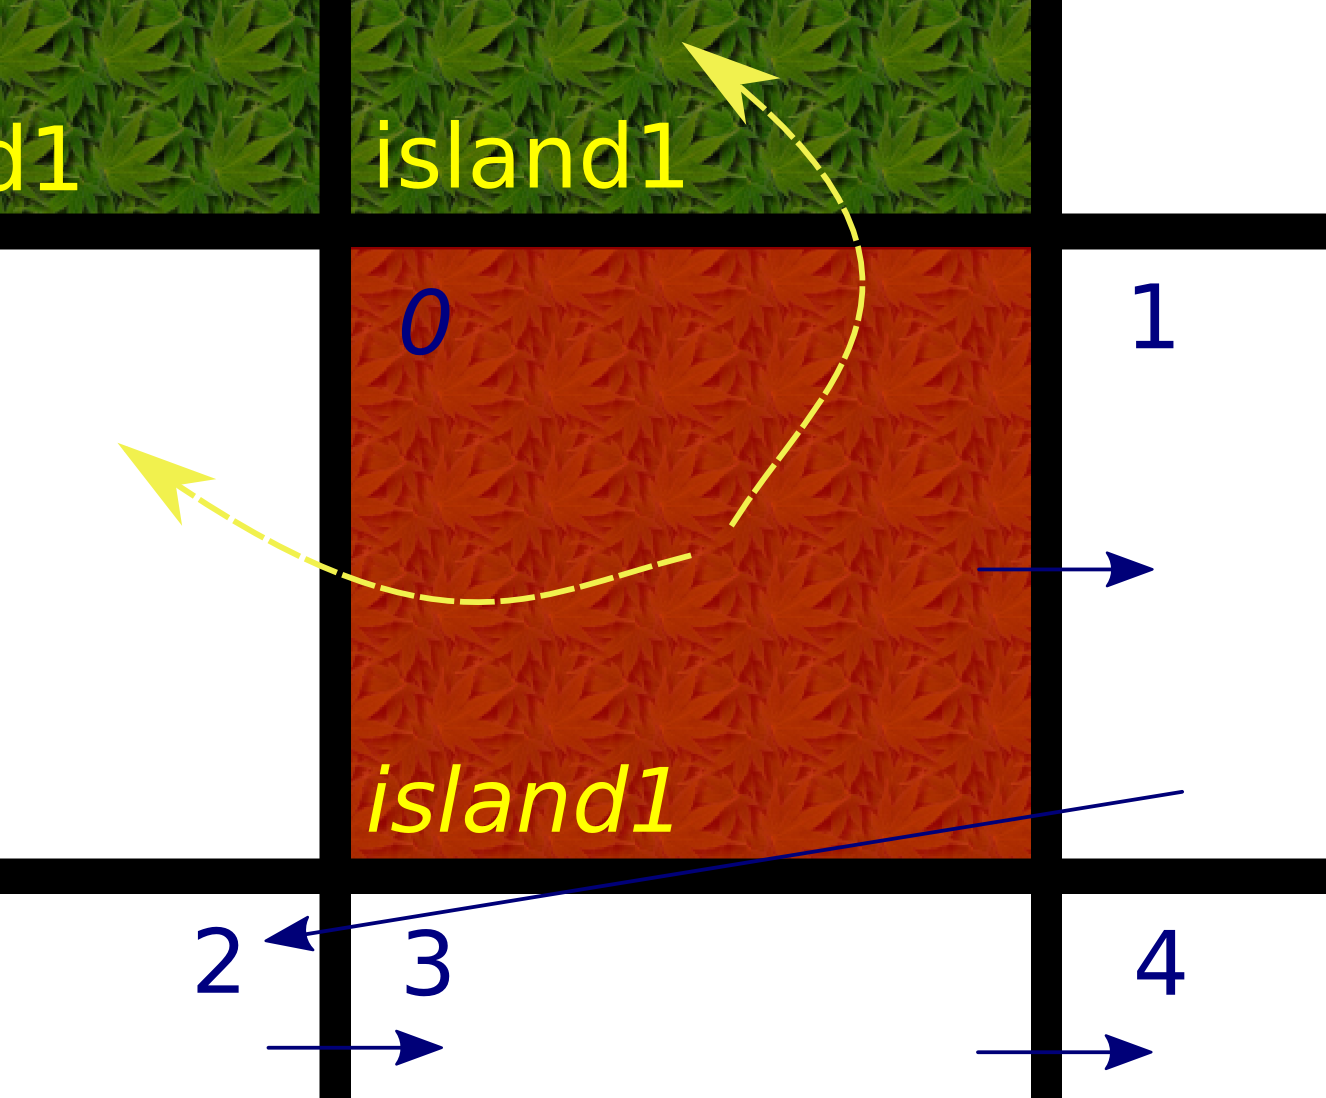
\includegraphics[width=0.7\textwidth]{gfx/merge_algorithm.png}

  \caption{Der Partitionierungsalgorithmus für die Islands. Die gelben Pfeile
  geben an, welche Gitterflächen auf das Vorhandensein von Tiles überprüft
  werden. Der Algorithmus traversiert die Tiles von oben links nach unten
  rechts (blau eingezeichnet).}
  \label{figure:automaton-intersection}
\end{figure}

Wie in Abschnitt \ref{kartenformat} erklärt, besteht die Schwierigkeit des
Transformationsprozesses in diese Richtung darin, zusammenliegende Bodentiles zu
erkennen. Dadurch benötigt das Speichern großer Inseln eine gewisse Zeit bis die
Gruppierung der Inslen beendet ist. Durch einige Performance-Optimierungen
konnte die Speicherzeit für eine Referenzkarte von über einer Minute auf fünf
Sekunden gedrückt werden.
